% !TeX spellcheck = en_US
\documentclass[french]{yLectureNote}

\title{Mécanique}
\subtitle{Mécanique du point}
\author{Paulhenry Saux}
\date{\today}
\yLanguage{Français}

\professor{S.Deheuvels}%sebastien.deveuhels.irap.omp.eu

\usepackage{graphicx}%----pour mettre des images
\usepackage[utf8]{inputenc}%---encodage
\usepackage{geometry}%---pour modifier les tailles et mettre a4paper
%\usepackage{awesomebox}%---pour les boites d'exercices, de pbq et de croquis ---d\'esactiv\'e pour les TP de PC
\usepackage{tikz}%---pour deiffner + d\'ependance de chemfig
\usepackage{tkz-tab}
\usepackage{chemfig}%---pour deiffner formules chimiques
\usepackage{chemformula}%---pour les formules chimiques en \'equation : \ch{...}
\usepackage{tabularx}%---pour dimensionner automatiquement les tableaux avec variable X
\usepackage{awesomebox}%---Pour les boites info, danger et autres
\usepackage{menukeys}%---Pour deiffner les touches de Calculatrice
\usepackage{fancyhdr}%---pour les en-t\^ete personnalis\'ees
\usepackage{blindtext}%---pour les liens
\usepackage{hyperref}%---pour les liens (\`a mettre en dernier)
\usepackage{caption}%---pour la francisation de la l\'egende table vers Tableau
\usepackage{pifont}
\usepackage{array}%---pour les tableaux
\usepackage{lipsum}
\usepackage{yFlatTable}
\usepackage{multicol}
\newcommand{\Lim}[1]{\lim\limits_{\substack{#1}}\:}
\renewcommand{\vec}{\overrightarrow}
\newcommand{\norm}[1]{||\vec{#1}||}
\DeclareMathOperator\arctanh{arctanh}
\begin{document}

%\titleOne
\setcounter{chapter}{5}
	\chapter{Oscillateurs}
	\section{Notion d'oscillateur}
	\subsection{Définition}
Tout système physique manifestant la variation d'une grandeur physique autour d'une position d'équilibre.

On les rencontre dans tous les domaines de la physique :Circuits électriques, pendule, ressort, corde de guitare, ondes acoustiques, mécanique quantique\dots
\subsection{Types}
\subsubsection{Oscillation périodiques}
Quand les variations se reproduisent à l'identique au cours du temps.

On défini la période $T$, la fréquence $\nu = \frac{1}{T}$ et la pulsation $\omega = \frac{2\pi}{T} = 2\pi\nu$
\subsubsection{Oscillateurs amortis}
Quand l'amplitudes des oscillations diminue au cours du temps, du fait, principalement de la dissipation de l'énergie.
\subsubsection{Types d'oscillation}
Elles sont \emph{libres} quand l'oscillateur oscille en fonction des ses propres caractéristiques : Ressort l\^aché

Elles sont \emph{forcées} : un autre système tente d'imposer une certaine fréquence d'oscillation au système.
\subsection{Ressort}
Un ressort est caractérisé par
\begin{itemize}
 \item sa longueur à vide $l_0$
 \item une constante de raideur $K$
\end{itemize}
La force de rappel $\vec{F_r}$ exercée par le ressort à une intensité proportionnelle à l'allongement du ressort. La constante de proportionnalité correspond à $K$ :
\[ - \vec{F_r} = k(x-l_0)\vec{e_x}\]

Pour connaître le signe, il faut représenter le cas d'un allongement positif et regarder dans quel sens est la force $\vec{F_r}$.

Souvent, on prend pour origine du repère la longueur à vide du ressort. Dans ce cas, l'allongement du ressort vaut $x$.

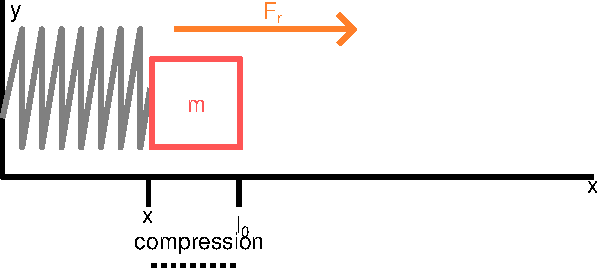
\includegraphics[scale=0.5]{compression}\: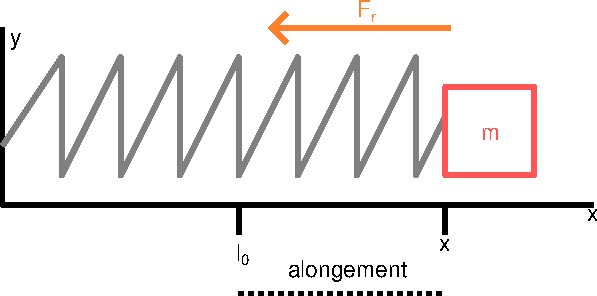
\includegraphics[scale=0.5]{alongement}

Mise en équation : Masse $m$ au  bout d'un ressort de constante $K$

Forces appliquées $(\vec{F_r},\vec{P},\vec{R}$ : On néglige les frottements : $\vec{R}\perp$ au déplacement.

\[m\vec{a} = \vec{F_r}+\vec{P}+\vec{R}\]
\[\left\{\begin{matrix}
 m\ddot{x} &= -kx \iff m\ddot{x} + kx = 0 \text{ : Oscillateur harmonique}\\
 m\ddot{y} &= -mg+R \iff R = mg\\
\end{matrix}\right.\]
\section{Oscillateur harmonique (OH)}
On appelle \emph{ocillateur harmonique} un système qui répond à l'EQD suivante :
\[\frac{\mathrm{d}^2x}{\mathrm{d}t^2}+ \omega_0^2x(t) = 0\]

Elle est du second ordre linéaire à coefficient constant sans terme du premier ordre.\marginInfo{Conditions nécéssaires : Si le coefficient du terme du second ordre est égal à 1, le coefficient du terme d'ordre 0 est positif}

Exemple : $\ddot{x}+4x = 0$ est un OH mais pas $\ddot{x}-x=0$

% \subsubsection{Formulation équivalente de l'OH}
% \begin{flalign*}
% \ddot{x}+\omega_0^2x=0\\
% \ddot{x}\dot{x}+\omega_0^2x\dot{x}=0\\
% \frac{\mathrm{d}}{\mathrm{d}t}(\frac{\dot{x}^2}{2}) + \omega_0^2\frac{\mathrm{d}}{\mathrm{d}t}(\frac{x^2}{2}) = 0 \\
% \frac{\mathrm{d}}{\mathrm{d}t}(\frac{\dot{x}^2}{2} + \omega_0^2\frac{x^2}{2}) = 0 \\
% \frac{\mathrm{d}}{\mathrm{d}t}(\frac{\dot{x}^2}{2}m + \omega_0^2\frac{x^2}{2}m) = 0 \\
% \frac{\mathrm{d}}{\mathrm{d}t}(Ec + Epp) = 0 \\
% Ec + Epp = Cst \\
% \end{flalign*}
\subsection{Résolution}
On cherche des solutions de la forme
\begin{flalign}
x&= Ce^{rt}\label{solution_generale}\\
\dot{x} &= Cre^{rt}\notag\\
\ddot{x} &= Cr^2e^{rt}\notag
\end{flalign}
On injecte \eqref{solution_generale} dans l'EQD pour obtenir l'équation caractéristique
\begin{flalign*}
r^2+\omega_0^2 &= 0\\
\iff r^2 &= -\omega_0^2\\
\iff r &= \pm i\omega_0
\end{flalign*}

La solution s'écrit donc \begin{equation}
x(t) = \underline{C_1}e^{-i\omega_0t} + \underline{C_2}e^{+i\omega_0t}\label{forme_1}
\end{equation}


Dans la pratique, l'expression \eqref{forme_1} n'est pas très utilisée car généralement $x(t)$ est une grandeur réelle. En fait, on peut aussi l'écrire sous la forme \[A\cos(\omega_0t) + B\sin(\omega_0t)\]
\begin{myproof}[Démonstration de la deuxième forme]
\begin{flalign*}
x(t) &= Re((a+ib)e^{-i\omega_0t} + (c+id)e^{i\omega_0t} )\\
&= Re((a+ib)(\cos(\omega_0t)-i\sin(\omega_0t) + (c+id)(\cos(\omega_0t)+i\sin(\omega_0t) ))\\
&= Re(a\cos(\omega_0t) - ia\sin(\omega_0t) + ib\cos(\omega_0t) + b\sin(\omega_0t)+c\cos(\omega_0t) +ic\sin(\omega_0t)+id\cos(\omega_0t)-d\sin(\omega_0t))\\
&= a\cos(\omega_0t)  + b\sin(\omega_0t)+c\cos(\omega_0t) -d\sin(\omega_0t))\\
&= (a+c) \cos(\omega_0t) + (b-d)\sin(\omega_0t)\\
&= A\cos(\omega_0t) + B\sin(\omega_0t)
\end{flalign*}
\end{myproof}
On peut aussi l'écrire sous la forme \[x(t) = C\cos(\omega_0t+\varphi) \text{ou }x(t) = D\sin(\omega_0t+\eta)\]

\begin{myproof}[Démonstration de la 3e forme]
\begin{flalign*}
C\cos(\omega_0t+\varphi) &= C\cos(\omega_0t)\cos(\varphi) - C\sin(\omega_0t)\sin(\varphi)\\
&= A \cos(\omega_0t) + B\sin(\omega_0t)
\end{flalign*}
\end{myproof}
Chacune des solutions fait intervenir 2 constantes d'intégration : $A$ et $B$, $C$ et $\varphi$, $D$ et $\eta$, que l'on détermine en appliquant les conditions initiales sur $x(t)$ et $\dot{x}(t)$.

\checkInfo{Exemple du ressort}{
La solution de l'EQD est $x(t) = A\cos(\omega_0t) + B\sin(\omega_0t)$

Si à $t=0$, on allonge le ressort sur uns distance $x(0) = x_m$ et on étudie le mouvement sans vitesse initiale ($\dot{x}(0) = 0$).

$x(0) = x_m = A\times 1$.

Il faut calculer $\dot{x}(t) = - A\omega_0\sin(\omega_0t) + B\omega_0\sin(\omega_0t)$, donc $\dot{x}(0) = B\omega_0 = 0$ car pas de vitesse initiale, donc $B=0$

On obtient alors $x(t) = x_m\cos(\omega_0t)$ et $\dot{x} = -x_m \omega_0 \sin(\omega_0t)$.}

\subsubsection{Période T des oscillations}
Il faut trouver $T$ vérifiant :
\begin{flalign*}
x(t+T) &= x(t)\\
x_m\cos(\omega_0(t+T))& = x_m \cos(\omega_0t)\\
x_m\cos(\omega_0t+\omega_0T) = x_m\cos(\omega_0t)\\
\omega_0T = 2\pi \Rightarrow \omega_0 \frac{2\pi}{T}\\
\end{flalign*}

Ici, $T = \frac{2\pi}{\omega_0} = 2\pi \sqrt{\frac{m}{k}}$

\subsubsection{Représentation graphique}
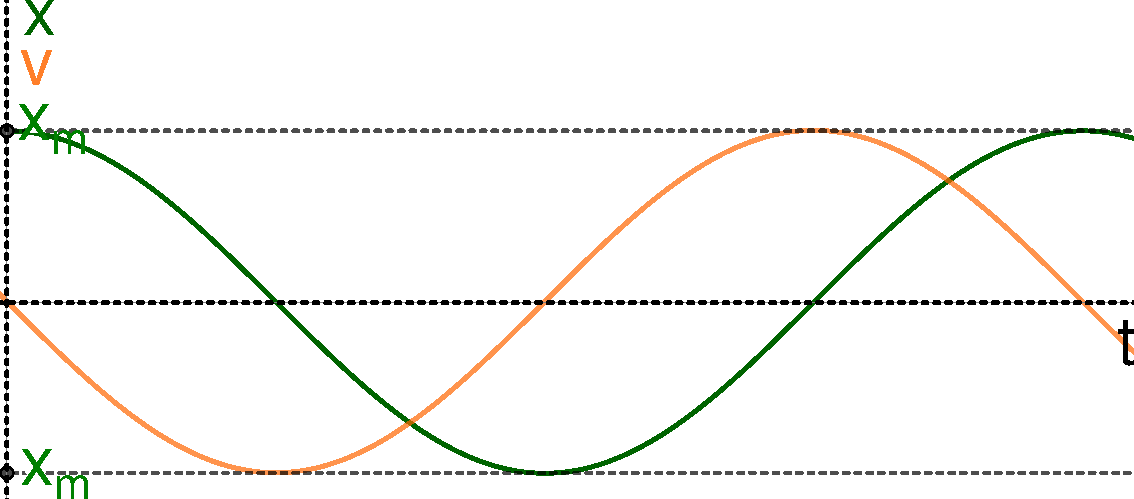
\includegraphics[scale=0.5]{representation_1}

Quand l'amplitude des oscillations est maximale, la vitesse est nulle et quand $x$ est nul, la vitesse est maximale.\marginInfo{Vitesse et position sont dits en quadrature de phase.}
\section{Oscillateurs amortis}
La solution d'un OH correspond à un mouvement perpétuel. Il s'agit d'un cas idéal sans dissipation d'énergie. Dans la pratique, il y a toujours une perte d'énergie. On parle alors d'amortissement de l'OH.
\subsection{Mise en équation}
On revient au cas du ressort étiré et on considère en plus une force de frottement fluide $\vec{F_f} = -\alpha \vec{v}$. On a toujours, à $t=0$, $x(0) = x_m$ et $\dot{x}(0) = 0$

Bilan des forces : $\vec{P},\vec{R},\vec{F_r},\vec{F_f}$.

On applique le PFD : $m\vec{a} = \vec{P}+\vec{R}+\vec{F_r}+\vec{F_f}$
\[\left\{\begin{matrix}
 m\ddot{x} &= 0 + 0 -kx -\alpha \dot{x}\\
 m\ddot{y} &= -mg+R + 0 -\alpha\dot{y}
\end{matrix}\right.\]

Pas de mouvement selon $y$, donc $y=\dot{y} = \ddot{y} = 0$
\begin{equation}\left\{\begin{matrix}
 m\ddot{x} &=-kx -\alpha \dot{x}\\
0 &= -mg+R + 0 \Rightarrow R = mg
\end{matrix}\right.\label{systeme_1}\end{equation}

On remarque que les forces de frottement ajoutent un terme du premier ordre. On obtient de \eqref{systeme_1} l'EQD
\begin{equation}\ddot{x} + \frac{\alpha}{m}\dot{x} + \frac{k}{m}x = 0\label{eqd_1}\end{equation}

On peut écrire \eqref{eqd_1} sous forme canonique, avec $\tau = \frac{m}{\alpha}$ et $\omega_0 = \sqrt{\frac{k}{m}}$ :
\begin{equation}\ddot{x} + \frac{1}{\tau}\dot{x} + \omega_0^2x = 0\label{eqd_1_h}\end{equation}

\subsection{Résolution}
\eqref{eqd_1_h} est homogène, on cherche des solutions sous la forme $Ce^{rt}$

L'équation caractéristique de \eqref{eqd_1_h} est : \begin{equation}r^2 + \frac{1}{\tau}r + \omega_0^2 = 0\label{eq_c_1}\end{equation}

\eqref{eq_c_1} est du second degré dont on calcule le discriminant ! \begin{equation}\Delta = \frac{1}{\tau^2} - 4\omega_0^2 = \frac{1}{\tau^2}(1-4\omega_0^2\tau^2)\label{delta}\end{equation} Cela fait intervenir la grandeur $Q = \omega_0\tau$ appelé \emph{facteur de qualité}, sans dimensions.
\subsubsection{Temps}
$\omega_0 = \frac{2\pi}{T}$ avec $T$ la période de l'OH, en l'absence de frottement

$\tau$ est le temps caractéristique sur lequel les frottements opèrent.

$Q = \omega_0\tau = 2\pi\frac{\tau}{T}$

Si $Q>> 1$, les frottements n'ont pas le temps d'agir pendant une période d'oscillation : on se rapproche de l'OH, car $\tau >> T$

Si $Q<<1 \iff \tau << T$, on s'attend à ce que les frottements emp\^echent les oscillations.
\subsection{Régimes}
On distingue trois cas suivants selon la valeur de $\Delta$ \eqref{delta}.
\criticalInfo{Calcul de $\omega$}{Ce n'est pas le $\omega_0$ initial mais une autre expression faisant intervenir $\omega_0$ !}
\subsubsection{Régime pseudo-périodique}
$\Delta < 0 $ si $1-4Q^2 < 0  \iff 4Q^2 > 1 $ou $Q > 0.5$.

Les racines de l'équation caractéristique \eqref{eq_c_1} sont
\begin{flalign*}
r &= \frac{-\frac{1}{\tau} \pm i\sqrt{4\omega_0^2-\frac{1}{\tau^2}}}{2}\\
&= -\frac{1}{2\tau} \pm \frac{i}{2}\sqrt{4\omega_0^2(1-\frac{1}{4\omega_0^2\tau^2})}\\
&= -\frac{1}{2\tau} \pm \frac{i}{2}\times 2\omega_0\sqrt{1-\frac{1}{4Q^2}}\\
&= -\frac{1}{2\tau} \pm i\times {\color{red}\omega_0\sqrt{1-\frac{1}{4Q^2}}}\\
&= -\frac{1}{2\tau} \pm i\times {\color{red}\omega_a}\\
\end{flalign*}
On a donc 2 racines : $r_1 = -\frac{1}{2\tau}-i\omega_a$ et $r_2 = -\frac{1}{2\tau}+i\omega_a$

La solution s'écrit alors
\begin{flalign*}
x(t) &= C_1e^{r_1t} + C_2e^{r_2t}\\
&= C_1e^{(-\frac{1}{2\tau}-i\omega_a)t} + C_2e^{(-\frac{1}{2\tau}+i\omega_a)t}\\
&= C_1 e^{-\frac{t}{2\tau}}e^{-i\omega_at}+C_2 e^{-\frac{t}{2\tau}}e^{+i\omega_at}\\
&= e^{-\frac{t}{2\tau}}(C_1e^{-i\omega_at} + C_2e^{+i\omega_at})\\
&= e^{-\frac{t}{2\tau}} (A\cos(\omega_at) + B\sin(\omega_at))\\
%&= e^{-\frac{t}{2\tau}} C\cos(\omega_at+\varphi)
\end{flalign*}
On détermine $A$ et $B$ avec les conditions initiales
\begin{flalign*}
x(0) &= x_m = A\\
\dot{x}(t) &= -\frac{1}{2\tau} e^{-t/2\tau} (A\cos(\omega_at) + B\sin(\omega_at)) + e^{-t/2\tau} (-A\omega_a \sin(\omega_at) + B\omega_a\cos(\omega_at))\\
&=  -\frac{1}{2\tau} x(t) +  e^{-t/2\tau} (-A\omega_a \sin(\omega_at) + B\omega_a\cos(\omega_at))\\
\dot{x}(0) &= -\frac{1}{2\tau} x(0) + B\omega_a
\end{flalign*}
Par énoncé, $\dot{x}(0) = 0$, donc $\frac{-x_m}{2\tau} + B\omega_a = 0 \iff B = \frac{x_m}{2\tau\omega_a}$

Tracé de la solution :

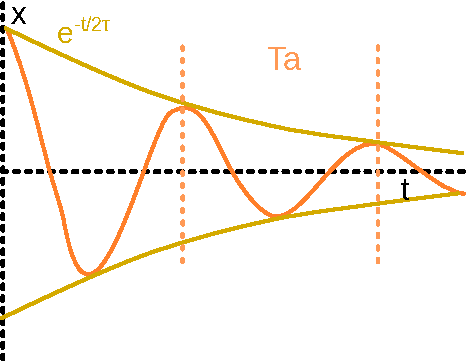
\includegraphics[scale=0.7]{pesudo}

On parle de pseudo-oscillations dont la période est $T_a = \frac{2\pi}{\omega_a}$

Dans le cas où $Q>>1$, $\omega_a = \omega_0\sqrt{1-\frac{1}{4Q^2}} \simeq \omega_0$ et $\omega_a \to \omega_0$, donc vers la pulsation de l'OH associée. Voir Graphe 6.4
\subsubsection{Régime apériodique}
$\Delta > 0 $ si $1-4Q^2 > 0  \iff 4Q^2 < 1 $ou $Q < 0.5$.

Les racines de l'équation caractéristique \eqref{eq_c_1} sont

\begin{flalign*}
r &= \frac{-\frac{1}{\tau} \pm \sqrt{-4\omega_0^2+\frac{1}{\tau^2}}}{2}\\
&= -\frac{1}{2\tau} \pm \frac{1}{2}\sqrt{4\omega_0^2(-1+\frac{1}{4\omega_0^2\tau^2}}\\
&= -\frac{1}{2\tau} \pm \frac{1}{2}\times 2\omega_0\sqrt{4\omega_0^2(-1+\frac{1}{4Q^2}}\\
&= -\frac{1}{2\tau} \pm  {\color{red}\omega_0\sqrt{-1+\frac{1}{4Q^2}}}\\
&= -\frac{1}{2\tau} \pm  {\color{red}\beta}\\
\end{flalign*}

La solution s'écrit alors
\begin{flalign*}
x(t) &= C_1e^{r_1t} + C_2e^{r_2t}\\
&= C_1e^{(-\frac{1}{2\tau}-\beta)t} + C_2e^{(-\frac{1}{2\tau}+\beta)t}\\
&= e^{-\frac{t}{2\tau}}(C_1e^{-\beta t} + C_2e^{+\beta t})\\
\end{flalign*}

Avec les conditions initiales, $x(0) = x_m$ et $\dot{x}(0) = 0$. De plus, $\dot{x}(t) = -\frac{1}{2\tau}x(t) + e^{-t/2\tau}(-C_1\beta e^{-\beta t} + C_2\beta ^{\beta t})$
\begin{equation}
\left\{\begin{matrix}
x(0) &= C_1+C_2 = x_m\\
\dot{x}(0) &= -\frac{x_m}{2\tau} + (C_2-C_1)\beta = 0
\end{matrix}\right.\label{systeme_2}
\end{equation}

On peut retrouver les $C$ en résolvant le système \eqref{systeme_2}

Tracé des solutions

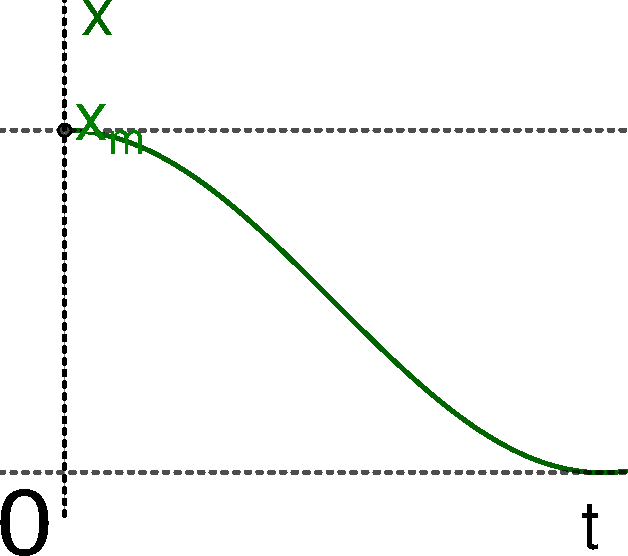
\includegraphics[scale=0.5]{aper}
\subsubsection{Régime critique}
$\Delta = 0 $ si $1-4Q^2 = 0  \iff 4Q^2 = 1 $ou $Q = 0.5$.

La racine double de l'équation caractéristique \eqref{eq_c_1} est
\begin{flalign*}
r &= \frac{-\frac{1}{\tau}}{2}\\
&= -\frac{1}{2\tau}
\end{flalign*}
La solution s'écrit alors : \marginCritical{Les constantes n'ont pas la m\^eme dimension. $C_1$ est une longueur et $C_2$ est une vitesse}
\begin{flalign*}
x(t) &= (C_1+C_2t)e^{-\frac{1}{2\tau}t}\\
&= C_1e^{-\frac{1}{2\tau}t} + C_2te^{-\frac{1}{2\tau}t}
\end{flalign*}
Avec les conditions initiales, $x(0) = x_m, \dot{x} = 0$, donc $C_1 = x_m$

$\dot{x}(t) = -\frac{C_1}{2\tau}e^{-\frac{1}{2\tau}t}+C_2e^{-\frac{1}{2\tau}t} - \frac{C_2}{2\tau}te^{-\frac{1}{2\tau}t}$

$\dot{x}(0) = -\frac{C_1}{2\tau} + C_2 \Rightarrow C_2 = \frac{C_1}{2\tau} = \frac{x_m}{2\tau}$

Donc $x(t) = x_me^{-\frac{1}{2\tau}t}(1+\frac{t}{2\tau})$.

Tracé de la solution

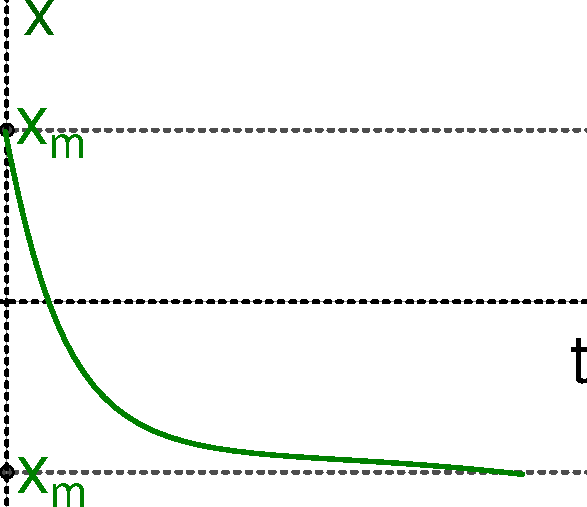
\includegraphics[scale=0.5]{delta0}
\subsubsection{Comparaison des solutions}
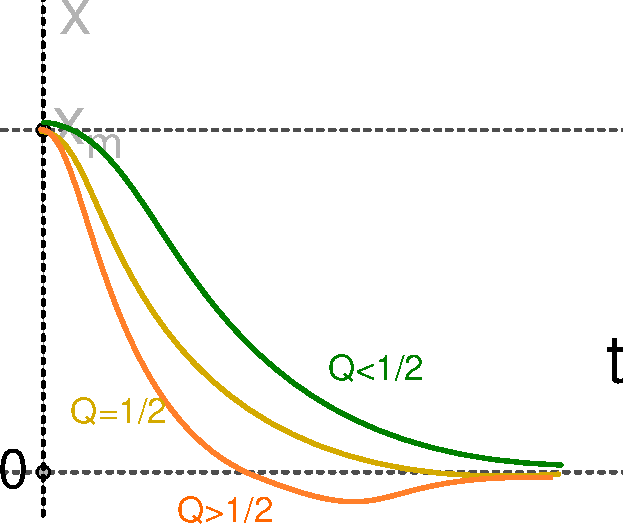
\includegraphics[scale=0.5]{compa}

Dans le régime critique, le retour à l'équilibre est le plus rapide. Il est donc intéressant pour étudier des amortisseurs
\end{document}

